\chapter{Принципи на реактивното програмиране}
\label{ch:reactive-programming-principles}

Едно от най-ранните описания на термина \emph{реактивни системи} в технически аспект е в публикацията на Дейвид Харел и Амир Пнуели от 1985-та година „\englishterm{On the Development of Reactive Systems}“ \cite{harel1985OnReactiveSystems}. В нея те разглеждат две противоположности — \emph{трансформиращи} и \emph{реактивни системи}. Трансформиращите системи приемат вход, трансформират го и генерират изход, с което те приключват. Реактивните системи, от своя страна, непрекъснато взаимодействат с външния свят и отговарят на идващия от него вход. Те не се ограничават само до компютърните системи, а се срещат навсякъде около нас. По-късно, през 1989-та година, Жерард Бери прави подобно разделение на три типа системи — \emph{трансформиращи}, \emph{интерактивни} (отделени от трансформиращите на Харел и Пнуели) и \emph{реактивни} \cite{berry1989RealTimeProgramming}. Трансформиращите системи работят върху предварително зададен вход и генерират резултат. Интерактивните системи взаимодействат с потребителите с темпо, определено от самите тях и в строго определена от тях последователност. Реактивните системи взаимодействат със средата със скорост, определена от самата среда. Харел и Пнуели допълнително развиват теорията си за описание и валидиране на такива системи \cite{harel1998ModelingReactiveSystems, manna1995ReactiveSystemsValidation}.

От тези публикации можем да извлечем следните характеристики на реактивните системи:

\begin{itemize*}
  \item във всеки един момент те трябва да могат да отговарят на вход от средата (съобразено с нейната скорост) \cite{harel1985OnReactiveSystems, berry1989RealTimeProgramming};
  \item всички взимодействия са най-често асинхронни, входът и изходът е непредвидим във времето и се случва конкурентно \cite{harel1998ModelingReactiveSystems};
  \item обикновено времето за реакция на системата е строго ограничено \cite{harel1998ModelingReactiveSystems};
  \item най-често се състоят от множество процеси, които работят конкурентно и паралелно \cite{manna1995ReactiveSystemsValidation, harel1998ModelingReactiveSystems};
  \item при декомпозирането им получените системи също биха били реактивни \cite{harel1985OnReactiveSystems};
  \item реалновремевите системи са най-често реактивни \cite{berry1989RealTimeProgramming, harel1985OnReactiveSystems}.
\end{itemize*}

По тези си характеристики програмирането на реактивни системи може да бъде разглеждано като вид \englishterm{dataflow} програмиране. Данните преминават през поток, започващ от асинхронен вход от външната среда, протичащ през подсистемите на реактивната система и достигащ обратно до външната среда като определен изход.

През 2013-та година Джонас Бонер и екип от разработчици публикуват „Манифест на реактивните системи“ (\englishterm{Reactive Manifesto}) \cite{reactiveManifesto}. В него се разглеждат принципи и добре познати архитектурни техники, чрез които да бъдат описани и постигнати характеристиките на реактивните системи в съвременната среда. През 2014-та манифеста бива обновен и изчистен допълнително. В тази дипломна работа ще използваме него за характеризиране на реактивните системи.

\section{Манифест на реактивните системи. Принципи}

Манифестът на реактивните системи дефинира тези системи като:

\begin{itemize}
  \item \emph{отзивчиви} (\englishterm{responsive}) — реагиращи на потребителите. Системата трябва да дава отговор на своите потребители до определено разумно време. Този отговор може да е както успешен резултат, така и съобщение за възникнала грешка или невъзможност за обработка. Така потребителите своевременно разбират какво е състоянието на системата и могат да реагират на това веднага, вместо да чакат дълго време без информация. Тук под потребители разбираме както крайни потребители, така и други системи, употребяващи услугата.
  
  \item \emph{устойчиви} (\englishterm{resilient}) — реагирaщи на грешки (\emph{failures}). Системата остава отзивчива дори в случаите на неочаквани грешки. Те биват изолирани възможно най-близо до тяхното възникване за да не бъдат разпространени до останалите части на системата. Системата, от своя страна, взима мерки да се поправи. Обикновено справянето с грешките бива делегирано към външни компоненти. Потребителят на услугата няма как да се справи с неочакваните грешки, поради което той не бива натоварен с тях. Липсата на устойчивост води до нарушаване на отзивчивостта на системата.
  
  \item \emph{еластични} (\englishterm{elastic}) — реагиращи на натоварване. Системата остава отзивчива, независимо от нейната натовареност. Системите могат реагират на промяна в скоростта на получаване на входни данни, като заемат или освободят налични ресурси. За целта е необходимо системите да бъдат вертикално и хоризонтално \emph{скалируеми} и да не съдържат критични точки.
  
  \item \emph{ориентирани около съобщения} (\englishterm{message-driven}) – реагиращи на вход. Компонентите на реактивните системи комуникират помежду си чрез асинхронни съобщения. Това води до слаба свързаност между компонентите и осигурява постигането на устойчивост и еластичност. Съобщенията позволяват изграждането на потоци от данни между компонентите и тяхното контролиране. Неблокиращата комуникация води до намалена и ефективна консумация на ресурси.
\end{itemize}

Всеки компонент от системата трябва да спазва разгледаните принципи. Това позволява те да бъдат композирани до по-големи системи.

Тези принципи пряко включват в себе си характеристиките, описани в началото на главата. На \shortlabeledref{фигура}{fig:reactive-trats} можем да видим зависимостите между тях.

\begin{figure}
  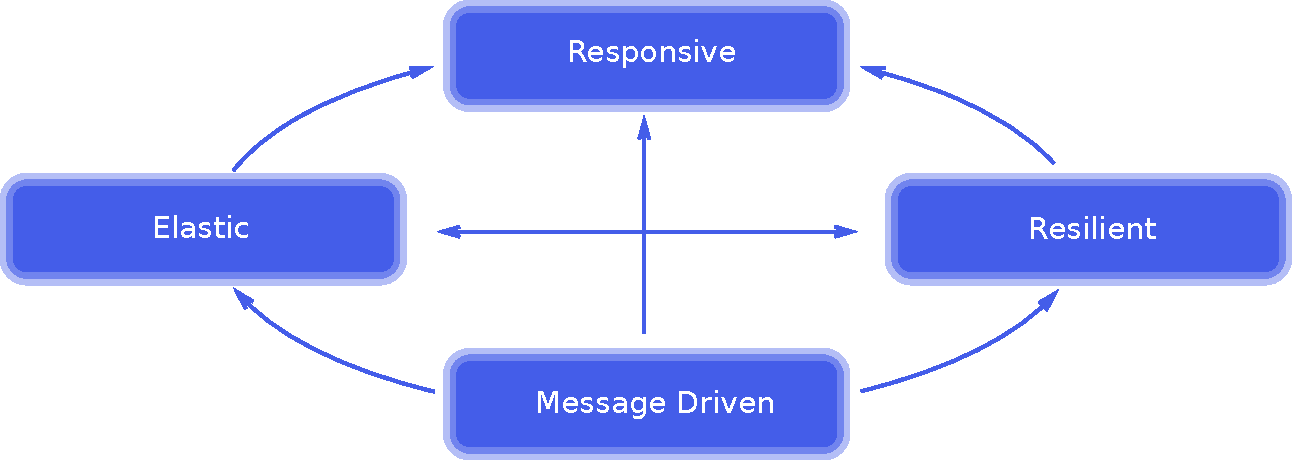
\includegraphics[width=\textwidth]{images/reactive-traits.pdf}
  \caption[Връзка между принципите на реактивните системи]{Връзка между принципите на реактивните системи (източник: \cite{reactiveManifesto})}
  \label{fig:reactive-trats}
\end{figure}

Преди да видим ползите от принципите и да разгледаме начини за тяхното постигане, нека да разгледаме и опишем проблемите на съвременните системи. В секциите след това ще видим как реактивните програми се справят с тях.

\section{Проблеми при съвременните системи}

\subsection{Архитектура}

Нека да разгледаме типичните особености на най-често срещаните съвременни системи. \shortlabeledref{Фигура}{fig:monolithic-architecture} представя архитектурата на едно типично монолитно уеб приложение.

\begin{figure}[th]
  \centering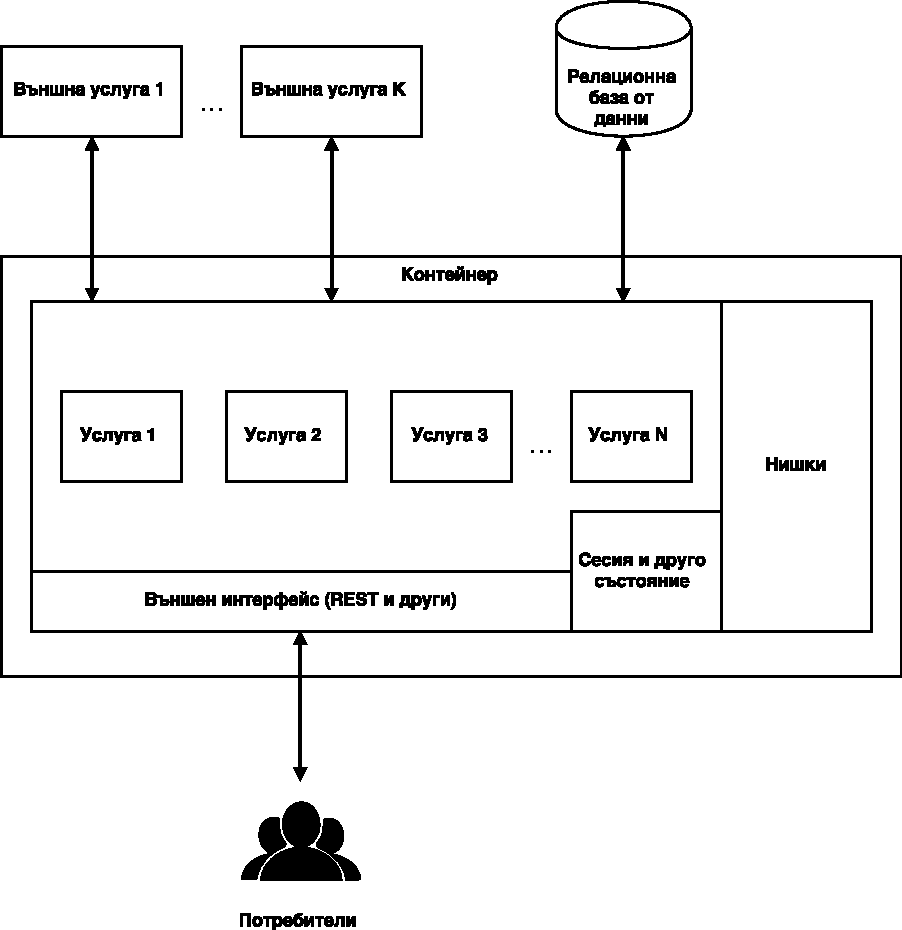
\includegraphics[width=0.8\textwidth]{images/monolithic-architecture.pdf}
  \caption{Архитектура на монолитна система}
  \label{fig:monolithic-architecture}
\end{figure}

Можем да отбележим следните характеристики:

\begin{itemize}
  \item Използване на централизирана релационна база от данни, осигуряваща строга консистентност на данните. Приложението изцяло разчита на това и борави с данните чрез CRUD\footnote{модел „създаване, четене, обновяване и изтриване“} модел.
  
  \item Наличие на силно свързани компоненти на ниво услуги. Те комуникират помежду си синхронно и си споделят наличните ресурси. Често услугите зависят от много други, като приемат, че всяка от тях отговаря мигновено и работи безгрешно. Липсва йерархична организация. Промяна в една от услугите или добавяне на нова изисква внедряване наново на цялото приложение.
  
  \item При грешка в някоя от услугите, извикващата я услуга е тази, от която се очаква да се справи с грешката. Така бизнес логиката бива преплетена с логика за справяне с грешки (различни от валидация). Неочакваните грешки се разпространяват навсякъде в системата и остават необработени.
  
  \item Използване на синхронна комуникация, както между локалните компоненти на приложението, така и с базата от данни и външни услуги, блокирайки текущата нишка. Поради това всяка една заявка към приложението бива обработена от различна нишка.
  
  \item Наличие на контейнер, който осигурява нишки за изпълнение на услугите на приложението при получаване на заявка и инициализира нейната обработка в някоя от наличните нишки, в която, в зависимост от заявката, се стартира компонент от слоя за външен интерфейс. При Java приложенията например това са контейнери като \englishterm{Apache Tomcat} и други.
  
  \item Съхранение на сесия и друга изменяема информация в приложението.
\end{itemize}

В следващите подсекции ще разгледаме проблемите, които възникват при тези характеристики.

\subsection{Разпределено програмиране. Синхронен модел}
\label{sec:synchronous-model}

Разпределените системи имат доста по-различни свойства от изпълняващите се на една машина. Тези свойства обаче често биват забравяни. През 1994-та Питър Дойч излага 7 заблуди за разпределените системи, които през 1997-та биват допълнени с 8-ма от Джеймс Гослинг \cite{deustch1994FallaciesOfDistributedComputing}:

\begin{enumerate*}
  \item Мрежата е надеждна.
  \item Времето за отговор (\englishterm{latency}) е нулево.
  \item Има безкраен \englishterm{bandwidth}.
  \item Мрежата е сигурна.
  \item Топологията не се променя.
  \item Има само един администратор.
  \item Цената за транспорт е нулева.
  \item Мрежата е хомогенна.
\end{enumerate*}

В разгледаните монолитни приложения обикновено тези заблуди и разлики биват пренебрегнати и комуникацията с отдалечени компоненти най-често бива третирана аналогично на локалните компоненти, осъществявана чрез синхронно извикване на функция. Този модел бива развиван още от ранните години на Интернет. В RFC 674 можем да открием предложение за т.~нар. „\englishterm{Procedure Call Protocol}“ \cite{rfc674}. Още тогава биват обсъждани и проблемите на този подход. RFC 684 изтъква като проблеми това, че отдалеченото извикване на функции има много по-висока цена и по-голяма вероятност за грешки, отколкото локалното, и че предаването на съобщения е по-добър модел за мрежова комуникация \cite{rfc684}. Въпреки това през годините се появяват различни модели в този стил, особено след развитието на ООП. Такива са например CORBA, DCOM, Java RMI и много други, където всичко се разглежда като синхронна комуникация между обекти, дефинирани от своя интерфейс, независимо от тяхното местоположение. В монолитните приложения по този начин се осъществява комуникацията с външни услуги или с базата от данни, които също са отдалечени. В публикацията „\englishterm{A Note on Distributed Programming}“ се разглеждат проблемите на тези модели и използването на разпределени обекти \cite{waldo1994ANoteOnDistributedProgramming}. Според авторите на публикацията — Джим Уалдо и други, те разчитат на следните три погрешни принципа:

\begin{itemize*}
  \item ООП дизайнът на дадено приложение не зависи от това как приложението ще бъде внедрено;
  \item възможността за грешки и производителността са свързани с имплементацията на компонентите и те не са важни за първоначалния дизайн;
  \item интерфейсът на един обект не зависи от това в какъв контекст той се използва.
\end{itemize*}

Авторите разглеждат следните причини за това, които са и част от заблудите, изложени от Питър Дойч:

\begin{itemize}
  \item \emph{времето за отговор} (\englishterm{latency}) при разпределените системи е много по-голямо. Локалното извикване на функция отнема от порядъка на наносекунда, докато изпращане на съобщение и получаване на обратен отговор по мрежата изисква стотици микросекунди в локална мрежа до стотици милисекунди в отдалечена и може да варира силно дори между последователни съобщения. Това може силно да сe отрази на производителността, ако някой алгоритъм изисква голяма доза комуникация между отдалечени компонентни. Също така важни споделени ресурси могат да се окажат заети прекалено дълго, което да навреди на скалируемостта. При синхронния модел е много лесно да бъде пропуснато, че зад даден метод стои отдалечено извикване.
  
  \item \emph{достъп до паметта} — отдалечените компоненти нямат достъп до паметта на другия компонент. Изпращането на съобщение изисква изпращане по мрежата на копие на всички данни в съобщението и обектите, които те реферират. При невнимание или ако програмистът не знае, че даден метод е отдалечен, това може да доведе до копиране на голямо количество данни или до неочаквани резултати от липса на споделена памет между компонентите.
  
  \item \emph{частични грешки} — и разпределените и локалните изчисления са податливи на грешки. При локалните системи тези грешки могат да бъдат открити веднага щом се случат, като най-често засягат всички участващи компоненти. При разпределените системи грешки могат да възникнат както в софтуера или хардуера на отдалечената машина, така и по трасето до нея. Тези грешки обаче няма как да бъдат уловени категорично — при липсата на отговор е възможно или системата все още да изчислява резултат или да се е получила повреда и задачата да не е била изпълнена напълно. Всички останали разпределени компоненти продължават работа, поради което грешката е само частична. При това е възможно да се получили неконсистентност между компонентите или отдалеченият компонент да остане в състояние, в което не може да продължи работа, за което е необходимо да бъдат предприети действия. Извикващият код единствен разбира за този недетерминизъм, евентуално чрез изключение за таймаут, и би могъл да опита да се справи с него. В резултат на това бизнес логиката на компонента бива преплетена с логика за справяне с недетерминистични грешки. Той рядко би могъл да се справи с тях успешно поради отдалечеността на извиквания компонент, поради което грешката се разпространява и в неговата система.
  
  \item \emph{конкурентност} — достъпът до отдалечените обекти е конкурентен по природа. Аналогично, това може да доведе до недетерминизъм и и извикващия код и отдалеченият обект трябва да могат да се справят с него.
\end{itemize} 

Според публикацията обратният модел — програмирането на локалните изчисления да следва това на разпределените, би направило програмирането твърде комплексно. Ще видим обаче, че когато направим това само на определени места в нашите програми, за които има смисъл компонентите да бъдат разпределени, този подход може да бъде доста естествен. Такива са различните реактивни подкомпоненти на реактивните системи. Актьорският модел, който ще представим в глава 4, е базиран на този подход.

При реактивните системи възможността за грешки е основен принцип, поради което те биват разглеждани на всеки един етап от дизайна на системата.

Прилагането на локален синхронен модел има за цел да улесни програмирането чрез скриване на сложността на проблема. Поради горните причини обаче тази сложност е \emph{съществена} \cite{brroks1987NoSilverBullet} и е част от природата на самия проблем. Опитът за нейното скриване скрива и проблемите, поради което те се проявяват неочаквано. В следващата глава ще видим кога всъщност е подходящо да скриваме сложността на проблема — т.~нар. инцидентна сложност, чрез абстракциите на функционалното програмиране, благодарение на което можем да ограничим по подходящ начин сложността на разпределените системи.

\subsection{Консистентност}
\label{sec:consistency-and-cap}

В предишната подсекция видяхме, че разпределеното програмиране има отражение върху консистентността на данните. Именно това е предмет на т.~нар. CAP теорема, представена от Ерик Брюър \cite{fox1999CAP} и по-късно доказана \cite{gilber2002CAP}. Тя гласи, че всяка разпределена система може да има най-много две от следните три свойства:

\begin{itemize*}
  \item \emph{строга консистентност} — всеки един възел в системата работи с едни и същи данни по едно и също време. Съществува тотална наредба между операциите, която води до това състояние;
  \item \emph{наличност} (\englishterm{availability}) — всеки работещ възел предоставя услуги си (например четене и писане) във всеки един момент;
  \item \emph{толерантност към деления} (\englishterm{partition tolerance}) — системата работи дори в случаите на частични грешки (загуба на съобщения, грешка във възлите и други), като те водят до временно или продължително разделение на възлите.
\end{itemize*}

Както вече видяхме, грешките във възлите на разпределените системи или в комуникацията между тях са неизбежно явление. Поради това толерантността към деления е желано свойство в системите. Така изборът обикновено пада между строга консистентност и наличност. Монолитните системи най-често се базират на строго консистентния ACID модел, което прави разпределението на тяхната база невъзможно без жертване на наличността на системата. Консистентността при разпределени системи изисква допълнително и съгласуване и синхронизация между всички възли при обновяване на данните, което, поради разгледаното в предишната секция, води до увеличено време за отговор \cite{lloyd2014CAPAndConsistency}, както и до намалена скалируемост (\shortlabeledref{секция}{sec:concurrency-threads-scalability}). Разпределените системи, които изберат наличността като основно свойство, използват по-слаби консистентни модели, които осигуряват много добра ефективност (\shortlabeledref{секция}{sec:dealing-with-consistency}).

От теоремата следва още, че съхраняваната сесийна информация не може да бъде споделена между различни реплики на монолитното приложение за да могат тези реплики да скалират и всяка да остане налична. Алтернатива е всяка реплика да съхранява собствена сесийна информация, но при грешка във възела това би могло да доведе до загуба на информацията и нетолерантност на системата към деления.

\subsection{Конкурентност, нишки и мютекси. Скалируемост}
\label{sec:concurrency-threads-scalability}

Монолитните приложения изискват използването на много нишки. Нишките обаче имат някои проблеми, както имплементационни, така и концептуални.

Нишките на популярните съвременни операционни системи и архитектури имат следните ограничения:

\begin{itemize*}
  \item стартирането на нишка е бавно;
  \item превключването между нишки (\emph{context switching}) е много скъпо. Всяко едно превключване изисква обработка от ядрото на операционната система, обновяване на състояние в ядрото, презареждане на голямо количество регистри в процесора, изпразване на неговия конвейер и нарушаване на предвиждащия му механизъм. Допълнително се извличат нови данни до кеша на процесора, тъй като старите най-често не са свързани с изпълнението на новата нишка;
  \item за всяка нишка е необходимо известно количество памет. В операционните системи Linux и Windows това е по подразбиране 1~MB виртуална памет за програмния стек (заемана физически на страници по 4~KB при нужда) и допълнителна памет за състоянието на нишката и процесорните регистри при превключване. При 32-битови системи 4000 нишки биха изчерпили цялото налично адресно пространство на един процес.
\end{itemize*} 

Операционните системи непрекъснато подобряват имллементациите (например верси 2.6 на Линукс чрез NPTL), но проблемите остават. Те се справят добре с малък брой нишки, но производителността започва да намалява при над няколко стотин, най-вече поради превключването между тях. Заради бавното стартиране приложенията поддържат множество от предварително стартирани нишки. Броят на нишките е балансиран, тъй като наличието на повече заявки към приложението, отколкото нишки има свободни, води до забавяне на заявките, а наличието на повече нишки се отразява на производителността и на заетата памет. Някои системи автоматично регулират множеството от нишки, в зависимост от натовареността.

Сериозен проблем е когато нишките се комбинират с блокиращи операции. Видяхме, че синхронния модел за комуникация до външни услуги и базата от данни води до блокиране на текущата нишка. Тя не може да продължи работа докато синхронното извикване не приключи, което отнема многократно повече време от локално извикване на функция (\shortlabeledref{секция}{sec:synchronous-model}). Така нишката остава да бездейства, заемайки ресурси без да извършва работа. Допълнително, блокирането изисква минимум две превключвания на контекста — в началото, когато нишката преминава в режим на покой, и в края, когато бива събудена обратно. Въпреки че нишката бездейства, тя все още натоварва планировчика на операционната система, поради това, че той трябва да обходи всички нишки и да избере готова за изпълнение. При обработването на заявка често се изисква повече от една комуникация с базата или външни услуги. Така за обработването само на една заявка, което обикновено в уеб приложенията се състои от трансфер само на няколко байта, се изисква продължително заемане на няколко пъти по-голямо количество памет (няколко килобайта физическа памет и 1~MB виртуална) и няколко превключвания на контекста. Не много на брой заявки могат бързо да натоварят системата и ресурсите ѝ. Повечето приложения трудно успяват да се справят с над 1000 заявки в секунда, с което силно се нарушава тяхната вертикална скалируемост.

Публикацията „\englishterm{The Problem with Threads}“ на Едуард Ли разглежда концептуалните проблеми на нишките \cite{lee2006TheProblemWithThreads}. Нишките представляват последователни процеси със споделена памет, базирани на императивен модел. Редът, в който всяка нишка достъпва тази памет (за четене и писане) е недетерминиран. Ако тези данни са изменяеми това води до недетерминирани резултати на всяка стъпка от изпълнението — ще разгледаме този проблем отново в \labeledref{секция}{sec:immutability}. За да докажем еквивалентнотта на две програми (или коректност на дадена програма) е необходимо да се изследват всички възможни комбинации за изпълнение, които най-често са много на брой. Нишките обикновено се използват със синхроназиционни примитиви, като мютекси, семафори, монитори и други, които значително намаляват възможните взаимодействия. Но на практика те не са достатъчни и при тяхното използване често остават труднооткриваеми възможни взаимодействия между нишките, които да доведат до \englishterm{deadlock}, \englishterm{race condition} или друг проблем. Сложността се засилва допълнително при многоядрените системи, където всяко ядро вижда различна версия на части от споделената памет и при промяна е необходимо тя да бъде допълнително съгласувана. В езика Java това става автоматично при използване на синхроназиционни примитиви, както и за променливите, дефинирани като \lstinline[language=Java]{volatile}, но е лесно да бъде пропуснато.

Хората трудно успяват да проследят конкурентността при нишките и трудно доказват твърдения за коректността на разглежданите програми, тъй като недетерминизмът е възможен във всяка една част от програмата. Същевременно хората всекидневно се справят с конкурентността във физическия свят без проблеми. Причината за тази разлика е, че нишките не моделират достатъчно точно физическия свят  \cite{lee2006TheProblemWithThreads}. Необходими са различни конкурентни модели, които не съдържат недетерминизъм по подразбиране, а такъв се въвежда само на определени контролирани места в програмите, където е необходимо. В тази дипломна работа ще разгледаме модели, базиращи се на поток от данни (което е в основата на реактивните системи), а не на контролен поток (постъпкови инструкции, на което се базират нишките), които моделират сравнително точно физическия свят.

Уеб приложенията обикновено делегират общата памет и синхронизацията към базата от данни, използвайки транзакции. Релационните транзакции обаче използват средства, подобни на синхроназиционните примитиви при нишки, които също са недетерминистични и водят до подобни проблеми. Често тези средства могат значително да натоварят базата или да блокират други заявки към нея, докато текущата се изпълнява. Така съответните нишки остават блокирани за по-дълго време, а пропускливостта на приложението се намалява.

Използването на синхроназиционни примитиви пречи на паралелното изпълнение на процесите на програмата. Синхронизирането по мютекс между няколко нишки позволява изпълнението само на една от тях в даден момент. Останалите нишки се блокират и приспиват, което се отразява по същия начин на производителността и скалируемостта както блокиране при отдалечено извикване. Допълнително, синхронизацията по мютекс изисква превключване към ядрото на операционната система и поддържане на списък от чакащи за мютекса нишки.

Влиянието на мютексите може да бъде тествано експериментално. В научната статия, представяща конкурентната опашка \englishterm{Disruptor}, можем да намерим подобен тест \cite{thompson2011Disruptor}. Статията тества последователно инкрементиране на 64-битово число 500 милиона пъти. При използване само на една нишка за стандартно постъпково инкрементиране операцията отнема 300 милисекунди. Ако нишката само заключва мютекс преди всяко инкрементиране, без да се бори с друга нишка, операцията нараства многократно до 10~000 милисекунди, поради съгласуван достъп до паметта. Ако в операцията се включат две нишки, всяка от които се бори за ключа на мютекса, операцията се забавя главоломно до 224~000 милисекунди, поради превключване между нишките и ядрото, което управлява синхронизацията.

\subsubsection{Скалируемост}

Синхронизацията и изразходването или неефективното използване на споделени ресурси (включително на централния процесор) може да доведе до липса на нишки и процеси, които да се изпълняват паралелно и ефективно във всеки един момент, с което изчислителната мощ на системата не бива оползотворена. Това представлява липса на вертикална скалируемост. Ефектът от това бива описан в \emph{законът на Амдал} \cite{amdahl1967Law}.

Нека $n \in \mathbb{N}$ е броят нишки (процеси), които се изпълняват паралелно, а $B \in [0, 1]$ е частта от програмата, която не може да бъде паралелизирана. Тогава ускоряването $S(n)$, което получаваме при изпълнение на програмата от $n$ паралелни нишки, е:

\begin{equation}
  S(n) = \frac{n}{1 + B(n - 1)}
\end{equation}

\begin{figure}
  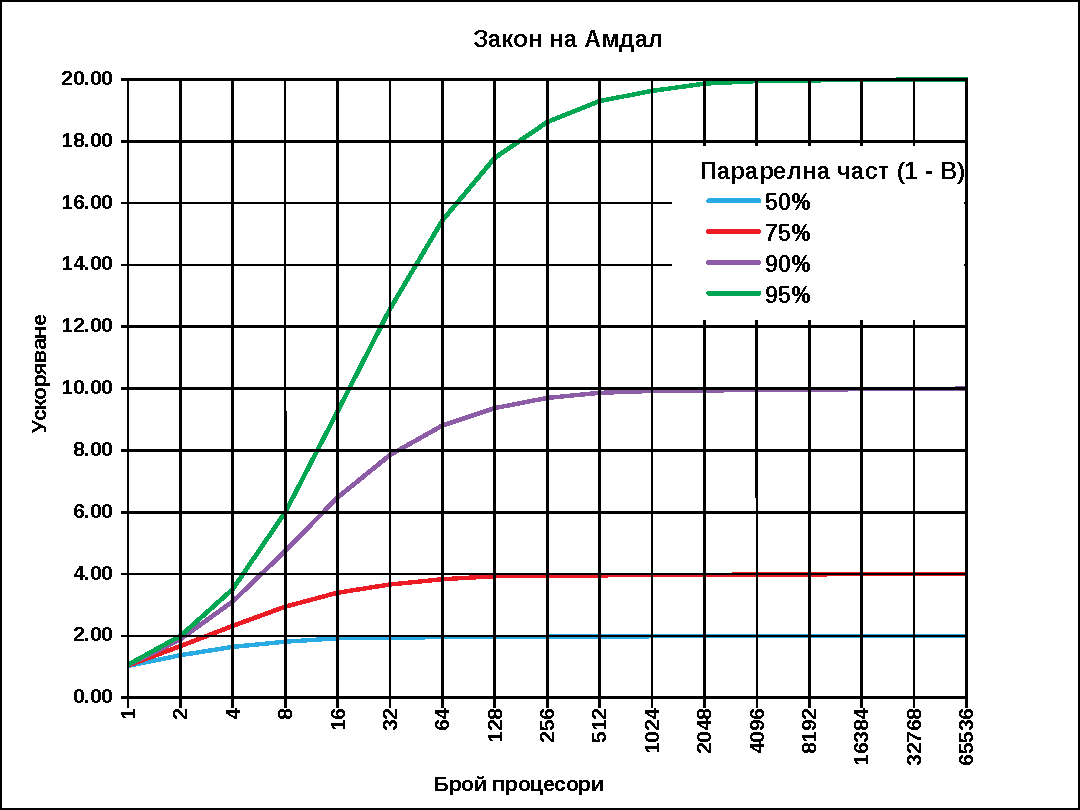
\includegraphics[width=\textwidth]{images/amdahls-law.pdf}
  \caption[Ускоряване по закона на Амдал в зависимост от броя на паралелните процеси]{Ускоряване по закона на Амдал в зависимост от броя на паралелните процеси (източник: \footnotesize\url{https://en.wikipedia.org/wiki/File:AmdahlsLaw.svg})}
  \label{fig:amdahls-law}
\end{figure}

\begin{figure}
  \centering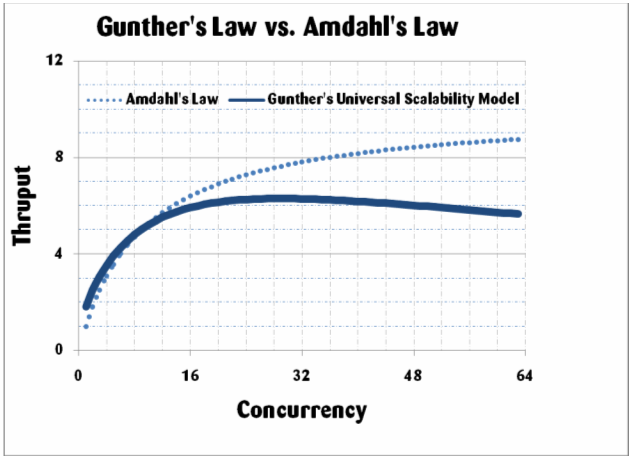
\includegraphics[width=0.75\textwidth]{images/gunthers-amdahls-laws.png}
  \caption[Сравнение между закона на Амдал и и универсиалния закон на скалируемостта при фиксирани параметри]{Сравнение между закона на Амдал и универсиалния закон на скалируемостта при фиксирани параметри (източник: \href{http://www.cmg.org/publications/measureit/2007-2/mit44/measureit-issue-5-09-a-review-of-beginning-excel-what-if-data-analysis-tools-getting-started-with-goal-seek-data-tables-scenarios-and-solver-by-michael-s-hines/}{Computer Management Group\\
      http://www.cmg.org/wp-content/uploads/2009/06/m\_44\_18b.png})}
  \label{fig:gunthers-law}
\end{figure}

\shortlabeledref{Фигура}{fig:amdahls-law} изобразява закона при различни стойности на паралелизация. При всяка от тях с увеличаването на броя на процесорните ядра системата скалира линейно до определен момент, след което плавно достига максимум. Дори при малки стойности на $B$ този максимум се достига бързо. При 95\% паралелизация възможното забързване е само 20 пъти, независимо от това колко паралелни процеса се използват.

През 1993-та година законът на Амдал бива допълнен от Нийл Гънтър. Гънтър включва още един важен параметър — необходимостта от съгласуване на споделените данни между различните процеси (между различните процесорни ядра) \cite{gunther1993Law}. Новият закон бива наречен \emph{универсиален закон на скалируемостта}.

Нека $n \in \mathbb{N}$ е броят нишки (процеси), които се изпълняват паралелно, $\sigma \in [0, 1]$ е частта от програмата, която не може да бъде паралелелизирана, а $\lambda \in [0, 1]$ е фактор, отразяващ времето, необходимо за съгласуване между процесите. Тогава ускоряването $S'(n)$, което получаваме при изпълнение на програмата от $n$ паралелни нишки, е:

\begin{equation}
S'(n) = \frac{n}{1 + \sigma(n - 1) + \sigma\lambda{n}(n - 1)}
\end{equation}

При $\lambda = 0$ получаваме закона на Амдал. На \shortlabeledref{фигура}{fig:gunthers-law} можем да видим сравнение на двата закона при $\sigma = 0.1$ и фиксирана $\lambda$. По закона на Гънтър скоростта не само спира да се увеличава от даден момент, ами при добавяне на още паралелни процеси дори намалява.

От тези закони можем да заключим, че дори малки непаралелизуеми части в програмата могат да имат голямо отражение върху скалируемостта на системата. Поради това е необходимо те да бъдат избягвани максимално, тоест да се намали синхронизацията и да се увеличи ефективността при използване на споделени изчислителни ресурси, като централния процесор. Лесно може да приложим законите и към разпределени системи за да характиризираме хоризонталната скалируемост, като например строго консистентните системи, разгледани в \shortlabeledref{секция}{sec:consistency-and-cap}.

\subsubsection{Междунишкова комуникация}

Важен аспект в системите е междунишковата комуникация. Тя обаче изисква синхронизация между нишките. Да разгледаме стандартната имплементация за предаване на задачи към множество от стартирани нишки. Това е класическият проблем производител/консуматор. Най-често той бива решаван чрез синхроназиционни монитори в двата края на опашка, съдържаща произведените обекти (в случая задачи за изпълнение). Както видяхме обаче, синхроназиционните примитиви имат висока цена \cite{thompson2011Disruptor}. В библиотеката Akka преди версия 2 се използва множество от нишки с такава имплементация. Реализацията не скалира при повече ядра (\shortlabeledref{фигура}{fig:fork-join-vs-thread-pool}), което практически илюстрира разгледаните закони. Такава имплементация се използва стандартно и в разглежданите монолитни приложения.

\begin{figure}
  \centering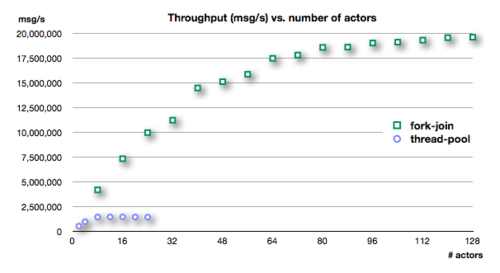
\includegraphics[width=0.75\textwidth]{images/fork-join-vs-thread-pool.png}
  \caption[\code{ForkJoinPool} срещу стандартен \code{ThreadPool} при 48 ядра]{\code{ForkJoinPool} срещу стандартен \code{ThreadPool} при 48 ядра. До 48 конкурентни актьора скалируемостта е сравнително линейна (източник: \cite{nordwall2012ForkJoin})}
  \label{fig:fork-join-vs-thread-pool}
\end{figure}

Ще разгледаме друг подход за предаване на данни между нишки. Той се нарича \englishterm{compare and swap} (CAS), което е стандартна инструкция в повече съвременни процесори. При тази операция при опит за промяна на дадена клетка от паметта промяната се извършва успешно само ако стойността ѝ съвпада с друга подадена на операцията стойност — очакваната текуща стойност в клетката. Сравнението изисква съгласуване между кешовете на изчислителните ядра, поради което операцията е по-бавна от стандартна промяна на клетка, но се извършва изцяло от процесора и не изисква превключване на контекста и обработка от ядрото на операционната система и не води до нарушаване на кеша. Стандартен начин за използване на CAS е т.~нар. „оптимистично заключване“, при което обновяването на клетка става в цикъл, при който на всяка итерация се прочита стойността на клетката, изчислява се нова стойност на нейна база, и се прави опит стойността да бъде записана чрез CAS. Цикълът продължава докато записът не е успешен. Поради липса на превключване на контекста операцията най-често приключва още в първите итерации, особено при системи с по-малко паралелни процеси. Освен това при този подход липсва блокиране, няма опасност за \englishterm{deadlock} и не се изисква поддържане на допълнителни структури, както при синхронизационните примитиви. При тест с инкрементационната задача от по-рано в секцията се наблюдава няколкократно по-добра производителност от синхроназиционните примитиви \cite{thompson2011Disruptor} (\shortlabeledref{таблица}{tab:synchronazation-performance}).

\begin{table}
  \centering
  \begin{tabular}{|l|r|}
    \hline
    {\bf Метод}             & {\bf Време (ms)} \\ \hline
    Единична нишка          & 300              \\ \hline
    Единична нишка с мютекс & 10~000            \\ \hline
    Две нишки с мютекс      & 224~000           \\ \hline
    Единична нишка с CAS    & 5~700             \\ \hline
    Две нишки с CAS         & 30~000            \\ \hline
  \end{tabular}
  \caption[Сравнение между различни синхроназиционни подходи]{Сравнение между различни синхроназиционни подходи (източник: \cite{thompson2011Disruptor})}
  \label{tab:synchronazation-performance}
\end{table}

При използване на CAS чрез разпределение на синхронизацията между няколко променливи могат да бъдат имплементирани доста ефективни скалируеми конкурентни структури, при които непаралелната част да е малка. Съществуват имплементации чрез CAS на конкурентни опашки без блокиране (като \code{ConcurrentLinkedQueue} в Java), които могат да бъдат използвани за по-ефективна имплементация на множества от нишки. Съществуват и имплементации на множества от нишки, които директно използват CAS по оптимален начин. Такава е \code{ForkJoinPool} от стандартната библиотека на Java, който (особено от версия 8 на Java) е силно оптимизиран за изпълнение на множество малки задачи. Akka от версия 2.0 използва именно него, с което постига почти линейна скалируемост (\shortlabeledref{фигура}{fig:fork-join-vs-thread-pool}) поради намаляване на превключванията на контекста от над 75~000 в секунда до около 1~000 в секунда \cite{nordwall2012ForkJoin}. CAS се използва често за ефективна междунишкова комуникация. Ефективни имплементации на \englishterm{Software Transanctional Memory} са възможни благодарение на тази операция.

Библиотеката на Java позволява директно използване на CAS чрез \code{AtomicReference} и други класове от пакета \code{java.util.concurrent.atomic}.

\subsection{Силно свързани компоненти}

Услугите вътре в монолитното приложение споделят ресурси и комуникират синхронно помежду си. Те са силно свързани и не могат да съществуват самостоятелно. Зависимостите между тях е трудно проследима, тъй като програмната среда не поставя ограничения върху това и обикновено липсват стриктни правила, които да бъдат следвани. Най-често липсват ясно определени граници между моделите и услугите на домейна и липсва йерархичност на услугите. Така едно евентуално разделение на приложението е трудно и сложно. Без ясни граници е и по-трудно работата по приложението да бъде разпределена измежду повече хора, които да работят сравнително независимо. Не е възможно отделни услуги да бъдат репликирани и скалирани самостоятелно и динамично, в зависимост от натоварване към тях. Репликиране на приложението може да се осъществи само чрез репликиране на целия монолитен блок (\shortlabeledref{фигура}{fig:monolithic-replication}), като всяка реплика използва една и съща инстанция на релационната база. Рядко се създават бази, отредени само за определена услуга.

\begin{figure}
  \centering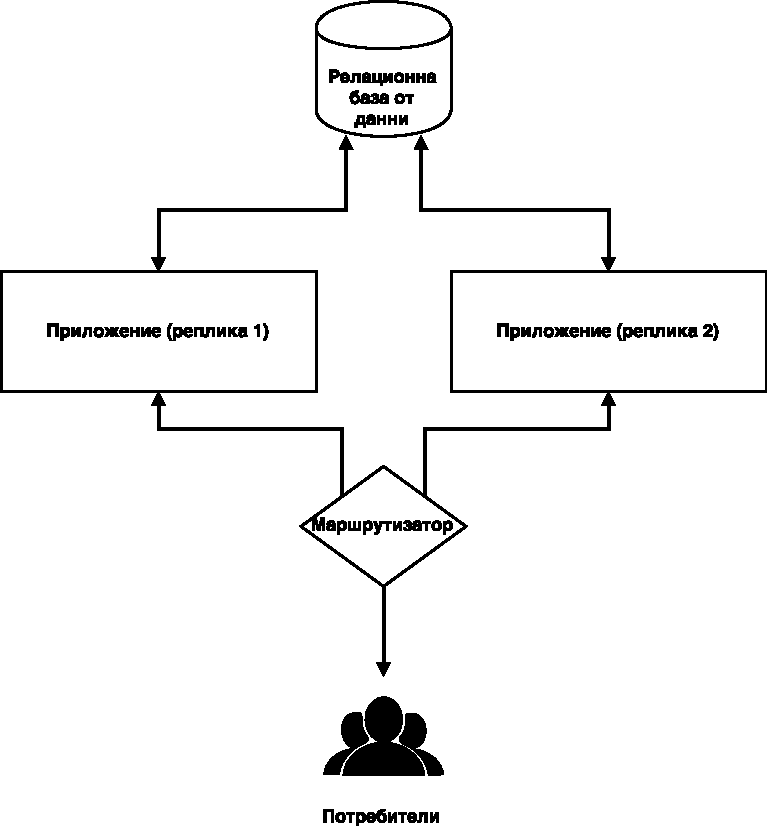
\includegraphics[width=0.8\textwidth]{images/monolithic-application-replication.pdf}
  \caption{Репликиране на монолитни приложения}
  \label{fig:monolithic-replication}
\end{figure}

Допълнително, синхронното извикване обвързва извикващия и извиквания компоненти. При локална комуникация извикваният код използва ресурсите на извикващия, а при отдалечена се блокира неговата нишка. Извикващият код спира работа докато извикваният не даде резултат, като не може да прави друго паралелно. Поради тези причини извикващият компонент е принуден да отговори възможно най-бързо за да може да освободи извиквания, вместо той сам да определи как оптимално и в най-подходящия момент да извърши операцията, например разпределяйки я в паралелни асинхронни изчисления. Така извикващият компонент е в контрол над извиквания, вместо последният да бъде самостоятелен. Стига се до това, че често в съвременните ООП езици обектите се изпълват с методи, които директно работят върху състоянието на обекта, без той да има право сам да реши дали, кога и как да извърши изискваната операция \cite{kuhn2015ReactiveDesignPatterns}. Такива са например всички \code{set} методи на Java обектите. Още една обвързаност на синхронния подход е, че при неочаквани грешки извикващият и извикваният компонент отказват заедно..

\subsection{Блокираща синхронна комуникация}

Във всяка от предишните подсекции видяхме как блокиращата синхронна комуникация се отразява негативно върху скалируемостта на системите, затруднява овладяването на грешки, подпомага тяхното разпространение, засилва свързаносста между компонентите и може да доведе до неочаквани ефекти. Освен това синхронният подход прави по-финното управление на комуникацията трудно. Можем да дадем следните два примера:

\begin{itemize}
  \item Често операциите изискват независима комуникация с други компоненти, чиито резултати да бъдат комбинирани. Поради това, че комуникацията е независима тя би могла да бъде извършена паралелно, което да ускори операцията. При синхронния модел обаче комуникацията се извършва последователно, всяко извикване се случва едно по едно. Единственият начин за паралелна комуникация с няколко компонента е стартиране на допълнителни нишки, които да извършат извикванията, и получаване на резултатите обратно в нишката на операцията. Това води до по-голяма сложност и до заемането на още допълнителни ресурси (при отдалечени компоненти всички изброени нишки ще бъдат блокирани, ще доведат до няколко превключвания на контекста и ще бъде синхронизирано връщането на резултат до оригиналната нишка). По-сложно комбиниране на многостъпкова комуникация с паралелни и последователни част е още по-трудно за реализация.
  
  \item Синхронният модел разчита, че отсрещният компонент е винаги готов да отговори. Възможно е обаче отдалечените компоненти да бъдат в състояние на повреда или да бъдат прекалено натоварени. Синхронният модел не предоставя начин за контролиране на комуникацията в такива случаи. Ако външна услуга или база от данни е засипана от заявки, с които не успява да се справи достатъчно бързо, при синхронния модел тези заяви не намаляват, а продължават да се увеличават със същото темпо, допълнително натоварвайки услугата, понякога водейки до срив. Същевременно забавените заявки водят до натрупване на заети ресурси и при извикващите компоненти, поради това че те стоят блокирани, което натоварва и техните подсистеми, а отговорът към потребителите се забавя многократно. Така натоварването или повреда в една част от системата се отразява на цялата система.
\end{itemize}

В следващите секции ще видим как комуникацията чрез асинхронни съобщения, напълно обратно на синхронния модел, подпомага скалируемостта и устойчивостта на системата и позволява доста по-голям контрол.

\section{Ориентираност около съобщения}

Съобщенията са в основата на реактивните системи. Те са обекти, които могат да бъдат явно управлявани от системата. Най-често биват организирани в управляеми опашки. Асинхронното предаване на съобщения не страда от проблемите на блокиращата синхронна комуникация, които разгледахме. Ще отбележим следните различия:

\begin{itemize*}
  \item предаването на съобщения няма семантиката на локалните извиквания. Не се изчаква то да завърши, а получаването на отговор е опционално, като се осъществява чрез получаване на ново асинхронно съобщение;
  \item изпращането на съобщения не води до заемане или блокиране на тежки ресурси, като нишки и други. След като съобщението е изпратено, компонентът свободно продължава работа;
  \item използването на съобщения води до слаба свързаност на компонентите. Получаващият компонент е свободен да избере как и кога да обработи съобщението оптимално, като дори може да го пропусне, ако е твърде натоварен. Компонентът изцяло енкапсулира състоянието си;
  \item съобщенията позволяват създаването на по-сложни протоколи за комуникация между компонентите;
  \item при блокиращата комуникация заявките се извършват една по една. Асинхронната комуникация позволява изпращане на поток от съобщения към друг компонент, паралелно изпращане на съобщения до няколко други компонента, както и други произволни комбинации. Потребителският код е свободен да управлява комуникацията според нуждите му;
  \item лесно е да бъде изградена двупосочна комуникация;
  \item получаването на съобщение за грешка няма как неочаквано да бъде разпространено в системата, както генерирането и хвърлянето на изключения;
  \item съобщенията могат да бъдат изпращани до няколко компонента и препредавани до различни компоненти и подкомпоненти.
\end{itemize*}

Важно е да отбележим, че за постигане на горните свойства и за избягване на част от недетерминизма съобщенията трябва да са неизменяеми обекти. Ще разгледаме неизменяемостта по-подробно в \labeledref{глава}{ch:functional-programming}. Недетерминизмът на разпределените системи се предава върху изпращането на отдалечени съобщения чрез неопределеността кога и дали съобщението ще бъде получено. При някои комуникационни протоколи е възможно и дублирано получаване на съобщението. Този недетерминизъм следва да бъде очакван при боравенето със съобщения. Възможно е явно изграждане на по-неефективни комуникационни канали, които да гарантират получаване на съобщението и липсата на дубликати след възстановяване от дадена повреда в системата, но те рядко оправдават цената си.

Комуникацията в Интернет е изцяло базирана на съобщения. Това показва, че те са подробно изследвани, скалируеми и ефективни при отдалечена комуникация. Успехът на Уеб се дължи именно на ориентираните около съобщения уеб протоколи (като HTTP). Тези протоколи са много подходящи за отдалечена асинхронна комуникация, като REST услугите са се превърнали в най-често използвания модел.

По семантика можем да разглеждаме три основни типа съобщения — \emph{събития},  \emph{команди} и \emph{информационни} съобщения:

\begin{itemize*}
  \item \emph{събитията} са съобщения, носещи информация за нещо случило се. Те могат да имат повече от един получател, като за изпращача не е важно как те ще бъдат обработени;
  \item \emph{командите} са съобщения, изискващи даден ефект да се случи. Получателят най-често е един, като изпращачът обикновено очаква да се наблюдава промяна или да бъде извлечен някакъв резултат;
  \item \emph{информационните} съобщения носят някаква информация на своя получател, без да определят как той да ги обработи. Такива са например съобщенията-отговори на заявки.
\end{itemize*}

Допълнително, самото получаване на съобщение представлява събитие от системата на получателя. Събитийните съобщения могат да бъдат използвани за мониторинг, събитиен вход и изход (секция 4.1), домейн събития и много други.

Като явни неизменяеми обекти, управлението на съобщенията може да бъде улеснено, а неговата сложност намалена, чрез подходящи функционални абстракции.

В следващите секции ще видим как асинхронните съобщения подпомагат всеки от другите реактивни принципи.

\section{Еластичност}

Всяка машина има определена максимална производителност и може да се справи само с определено натоварване. При по-голямо потребление е необходимо системата да бъде разпределена до повече изчислителни машини или към машината да бъдат добавени изчислителни ресурси. Същевременно използването им е скъпо, а потреблението се променя динамично. Бихме искали при намаляване на натоварването да спестим излишни средства и системата отново да бъде скалирана до по-малко машини и ресурси. Това свойство се нарича еластичност. За постигането му е необходимо системите да могат да бъдат скалирани, както хоризонтално, така и вертикално, и да бъдат изградени компоненти за мониторинг на натовареността и управление на ресурсите.

Вече видяхме, че за да постигнем вертикална скалируемост е необходимо да не бъдат излишно задържани изчислителни ресурси. Съобщенията подпомагат това. Получаващият компонент може да избере как оптимално да използва ресурсите, с които разполага, и да скалира обработката върху тях. За скалируемост е необходимо още да бъдат сведени до минимум непаралелизуемите части на системите. Това зависи от имплементацията на отделните компоненти и услуги. Тези услуги след това могат да бъдат репликирани в зависимост от нуждата от тях. За целта е необходимо услугите да бъдат разделени, така че всяка да може да бъде репликирана и скалирана самостоятелно. Това е възможно благодарение на слабата свързаност, която съобщенията осигуряват. Най-честият подход е т.~нар. \emph{прозрачност на местоположението} (\englishterm{location transparancy}). При него всяка инстанция на компонент получава адрес, като изпращането на съобщение до даден адрес изглежда еднакво, независимо от местоположението и от това дали компонента е локален или отдалечен. Така получаваме разпределен програмен модел дори за локалните компоненти. Допълнително тези адреси могат да бъдат изпращани като съобщения до всеки друг компонент. Така можем да скалираме услугите без за използващите ги компоненти да има значение местоположението им и това коя реплика използват. Свързването с реплика често се осъществява чрез компонент-маршрутизатор, който препредава съобщението към някоя от репликите.

Използването на прозрачност на местоположението позволява също така локалните компоненти лесно да бъдат разпределени при необходимост, без промяна на използващия ги код. Така разпределението на услугите по възли може да бъде лесно променяно и базирано на реални тестове.

Разделението на услугите позволява още определяне на ясни зависимости между тях, както и на йерархична структура на компоненти и подкомпоненти. Схемата на внедряване (разпределението на услугите) обикновено следва тази структура.

Важен въпрос е колко паралелни реплики са необходими при дадена натовареност на системата. Целта ни е обработката на всяко пристигнало съобщение да започне почти веднага. В противен случай консумирането на съобщения би било по-бавно от получаването им, което води до постепенно увеличаване на опашката със съобщения. С това се увеличава и времето за отговор на всяко едно съобщение. За установяване на този брой можем да използваме закона на Литъл \cite{little1961LawProof}.

Да разгледаме формулировка на закона за нашия проблем. Нека $\lambda$ е средната скорост, с която съобщенията се трупат в опашката (заявки/секунда), а W е средното време, необходимо за обработка на едно съобщение. Тогава средния брой съобщения $L$, които трябва да бъдат обработвани паралелно за да може опашката да не се препълва, се дава с формулата:

\begin{equation}
L = \lambda W
\end{equation}

Литъл нарича това стабилно състояние на процеса. Времето за отговор на едно съобщение включва времето за обработката му и времето за престой в опашки.

Броят съобщения в секунда зависи от натовареността на услугата, а средното време за обработка може да бъде установено експериментално. По-точно е обаче и двете величини да бъдат наблюдавани по време на изпълнение, тъй като могат да се променят. Можем да въведем компонент, който да наблюдава потока от съобщения или периодично да получава статистики за времето на обработка и натовареността от репликите. Така той може да пресметне $L$ и автоматично да скалира услугата при достигане на определена горна или долна граница. Добра практика е да бъде оставен резерв от реплики, които да поемат внезапно увеличение на натоварването докато скалирането се извършва. При йерархично разделение тази роля може да се поеме от родителския компонент на репликираната услуга.

\section{Устойчивост}

Във всяко едно приложение могат да се получат грешки. Колкото и добре да е написано то, в него винаги има бъгове. Допълнително видяхме и недетерминизма, който носи разпределената среда, и възможността за грешка в хардуера, софтуера или в комуникацията между възлите. Така грешките са сигурно явление в софтуерните системи. Затова реактивните системи трябва да бъдат толерантни към тяхното възникване, но освен това те трябва да могат да предприемат действия за възстановяване от грешките, за да могат да работят отново на пълен капацитет.

Основен подход за предпазване на важни компоненти и данни е тяхното репликиране и изолиране. Грешките често се разпространяват локално (повреда в комуникацията, спиране на електрозахранването, административни грешки и други), затова за да бъдат предпазени от разпространение им репликите трябва да бъдат изолирани в различни помещения и дори различни сгради или градове.

Когато дадена услуга на системата не работи, останалите услуги на реактивните приложения трябва да могат да продължат работа и евентуално да дават частични отговори, ако зависят от нея, стига това да има смисъл. Клиентските приложения трябва да приемат възможността за това и да деактивират компоненти при нужда, съобщавайки на крайните потребители, че услуга не е налична.

Една от най-честите причини за възникване на грешки е претоварването на отделни компоненти и услуги. Затова е важно системите да прилагат решения за предпазване от това. Ще разгледаме три основни мерки:

\begin{itemize*}
  \item \emph{изполване на ограничени опашки} — ако паралелизирането на някоя услуга не е достатъчно, тогава в използваните опашки ще започнат да се трупат съобщения, а паметта, която те заемат, да нараства. Това ще доведе до запълване на паметта на системата и нейния срив. Някои реактивни платформи, като Erlang, предпазват системата от това, като ограничават наличната памет за всеки компонент. Не всички системи имат това свойство обаче. Затова на критичните места, където могат да се трупат съобщения, трябва да бъдат използвани явни ограничени опашки, които да не допускат повече съобщения;
  \item \emph{временно прекъсване на потока към услуга, при зачестяване на съобщенията за грешки от нея} — не всяка услуга е предпазена по горния начин, но дори да е самото изпращане на съобщение до нея също натоварва системата. Можем да имплементираме механизъм при потребителите на услугата, който да следи за зачестили съобщения за грешка и да прекъсва потока към нея, когато те надхвърлят определена граница, до нейното възстановяване. Ще разгледаме механизъм, наречен \emph{прекъсвач на веригата} (\englishterm{circuit breaker}), чрез който може да бъде реализирано това. Механизмът би могъл да бъде подпомогнат, ако натоварената услуга връща съобщения за грешки възможно най-бързо (ще разгледаме това в \shortlabeledref{секция}{sec:responsive});
  \item \emph{контролиране на потока, идващ от даден компонент} — реактивните системи позволяват високоскоростно предаване на поточни данни между два компонента. Когато обаче получаващият компонент не успява да обработи съобщенията достатъчно бързо, той бива претоварен. За справяне с това е необходим механизъм, чрез който компонентът да сигнализира динамично какъв поток може да поеме и предаващият компонент да регулира скоростта в зависимост от това. Ще разгледаме механизъм за това в секцията за реактивни потоци.
\end{itemize*}

Всеки от разгледаните подходи се подпомага от характеристиките на съобщенията и тяхната възможност за явен контрол.

При синхронната комуникация видяхме, че извикващите компоненти няма как да се справят с неочакваните грешки в системата. Затова при реактивните системи ще разделим тези отговорности и ще въведем компонент, наречен \englishterm{supervisor}, който да следи състоянието на дадени компоненти. При възникване на грешка \englishterm{supervisor} компонентът получава грешката като съобщение и може да реши какви мерки да предприеме за възстановяване на дефектиралия компонент, или ако няма достатъчно информация да предаде грешката към по-външен \englishterm{supervisor}. Допълнително, може да бъде наблюдавана наличността на компонента чрез постоянно следени с \englishterm{ping} съобщения. При използване на прозрачност на местоположението компонентите могат да бъдат рестартирани, запазвайки адреса си, без това да се отразява на използващите ги компоненти.

При този механизъм за наблюдение логиката за справяне с грешки вече не е преплетена с бизнес логиката, ами е отделена на едно място. При йерархично разделение естествен кандидат за \emph{supervisor} са родителите на компонентите.

\section{Отзивчивост}
\label{sec:responsive}

Крайната цел на реактивните принципи са отзивчиви системи — системи, които отговарят винаги, когато това е възможно, и то в разумно време, независимо дали с резултат или грешка. За постигане на това е необходимо системата да бъде устойчива на различни повреди, за да може тя да продължи работа. Вече видяхме подходи за това. Необходимо е още всеки един отговор да бъде получаван бързо и за ограничено предсказуемо време.

За ускоряване на времето за отговор може да използваме различни подходи, повечето подпомагани от вече разгледаните реактивни принципи:

\begin{itemize*}
  \item паралелизация на комуникацията с услуги — така времето за отговор ще се намали до най-бавната от заявките, а не до сумата от всяка от тях. Използването на съобщения ни позволява този подход да бъде извършван лесно;
  \item видяхме, че при недостатъчен брой на паралелно обработващи компоненти по закона на Литъл, съобщенията започват да се трупат в опашката и времето за техния отговор се увеличава. Системата трябва автоматично да скалира, в зависимост от нуждите за паралелилизъм;
  \item в случаите когато паралелизма не е достатъчен, използването на ограничени опашки, което разгледахме, позволява изхвърляне на новодошлите съобщения, тъй като те няма да бъдат обработени достатъчно бързо. За всяко от тях можем веднага да пратим отговор за грешка, вместо той да се чака неограничено, като така получаваме съкратено време за отговор;
  \item аналогично, при използване на прекъсвач на веригата или подобен механизъм, можем веднага да изпратим съобщение за грешка;
  \item времето за отговор може да се намали и чрез използване на подобрени алгоритми.
\end{itemize*}

В някои случаи на повреда или при забавяне на системата няма да получим отговор достатъчно бързо. Както вече споменахме, двата случая не могат да бъдат различени. Съобщенията ни позволяват да следим колко се забавя даден отговор. Необходимо е да поставим горна граница, след която да приемем, че операцията е безуспешна и да върнем отговор за грешка. За определянето на тази граница е необходимо експериментално тестване на разпределението на времето за отговор на услугата и избор на подходяща стойност, така че почти всички заявки да са успешни, но стойността да е достатъчно ниска. Роланд Кун и Джейми Алън разглеждат този проблем \cite{kuhn2015ReactiveDesignPatterns}. Важно е също така да бъдат използвани алгоритми, които да имат предсказуемо време за отговор.

\section{Справяне с консистентността. Домейн модели}
\label{sec:dealing-with-consistency}

В \shortlabeledref{секция}{sec:consistency-and-cap} видяхме, че строгата консистентност е неефективна в разпределена среда и невъзможна, ако системата е налична постоянно. Съществуват обаче по-слаби формулировки на консистентност, които се вписват добре в разпределените системи. Такива са \emph{евентуалната} и \emph{причинната} консистентност. Евентуалната консистентност гарантира, че след промяна на определени данни промяната ще бъде видима от всички възли на системата до определено ограничено време, стига те да не бъдат променяни отново. През това време потребителите на останалите възли е възможно да виждат по-стара версия на данните. Причинната консистентност засилва евентуалната, гарантирайки частична наредба на операциите. Тя предпазва от това дадени операции да бъдат видими преди други в останалите възли, въпреки че са се случили по-късно, но е по-трудна за постигане. В тази дипломна работа ще разглеждаме евентуалната консистентност.

Реактивните системи често имат по-сложен домейн, който е трудно да се опише в CRUD термини. Основния проблем на CRUD е, че характеризира промените, които трябва да бъдат направени върху определени данни, но не и истинското действие на потребителя, от което те са породени. Вместо това можем да въведем собствени операции, определени от домейна, които да описват това действие. Тези операции можем да използваме в комбинация с \englishterm{Command Query Responsibility Segregation} (CQRS, отделяне на изменящите команди и заявките в различни модели), с което по-лесно можем да постигнем евентуална консистентност. Допълнително можем лесно да пазим хронология с всяка от тези операции, което да ни позволи възстановяване на системата към всеки един момент при евентуален срив, преповтаряне на операциите при бъг в програмата, както и извличането на допълнителна информация от действията на потребителите, ако такава се окаже необходима. Този подход се нарича \englishterm{event sourcing}.

Всички тези характеристики на реактивните системи се вписват добре в концепциите на \englishterm{Domain-Driven Design} (DDD) \cite{evans2003DDD}. При него домейните биват моделирани именно с операции, съответстващи на реалните действия на потребителите. DDD подражава на използването на неизменяеми обекти и други принципи от функционалното програмиране. DDD разделя домейна на различни \emph{ограничени контексти}, които съществуват самостоятелно и комуникират помежду си ограничено. Това съвпада с естественото разделение при реактивните системи на множества от компоненти и подуслуги, предоставящи дадена услуга, които са самостоятелни и комуникират помежду си чрез асинхронни съобщения.

\begin{chapterend}
  В следващата глава ще разгледаме функционалното програмиране като средство за изграждане на преизползваеми абстракции, с които да бъде контролирана сложността, породена от особеностите на реактивните системи. Ще разгледаме и неизменяемостта като основен принцип на функционалното програмиране за намаляване на недетерминизма и избягване на труднопроследимите странични ефекти.
  
  В глава 4 ще разгледаме различни реактивни средства и имплементации.
\end{chapterend}
